\documentclass[10pt,a4paper,oneside]{book}

\begin{document}

\chapter{Laboratory Instructions}

\section{Description of the Microscope}

The microscope is an Abbelight SAFe 180. It consists of an Olympus IX83 microscope, an Abbelight scanning illumination system, a Hamamatsu ORCA-Fusion digital CMOS camera, and other components. Some of these components are labeled in \autoref{fig:microscope} and \autoref{fig:electronics}.

\begin{figure}[ht]
    \centering
    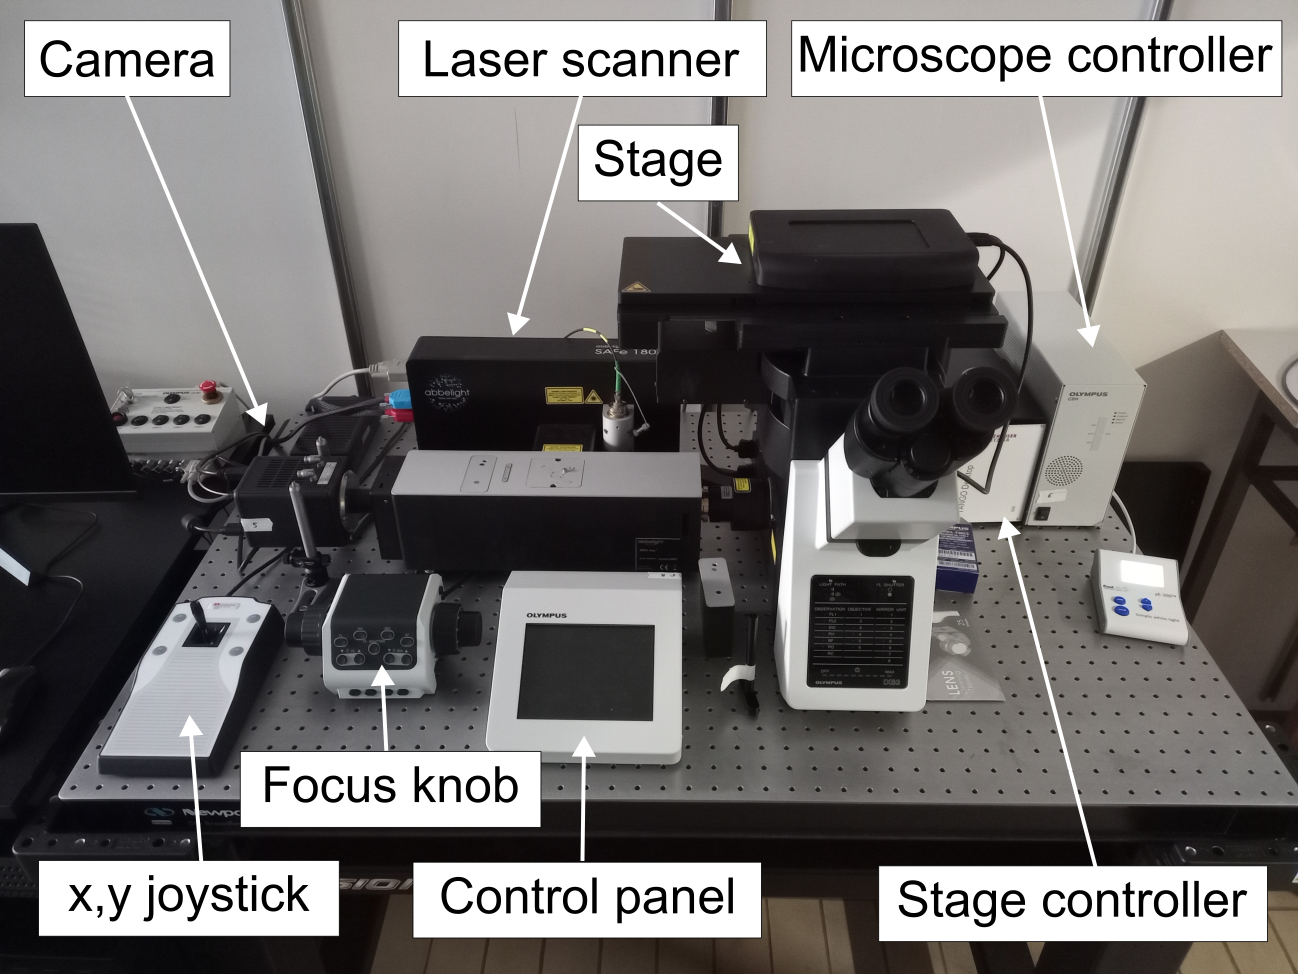
\includegraphics[width=0.75\textwidth]{microscope.png}
    \caption{The primary components of the microscope used in this course.}
    \label{fig:microscope}
\end{figure}

\begin{figure}[ht]
    \centering
    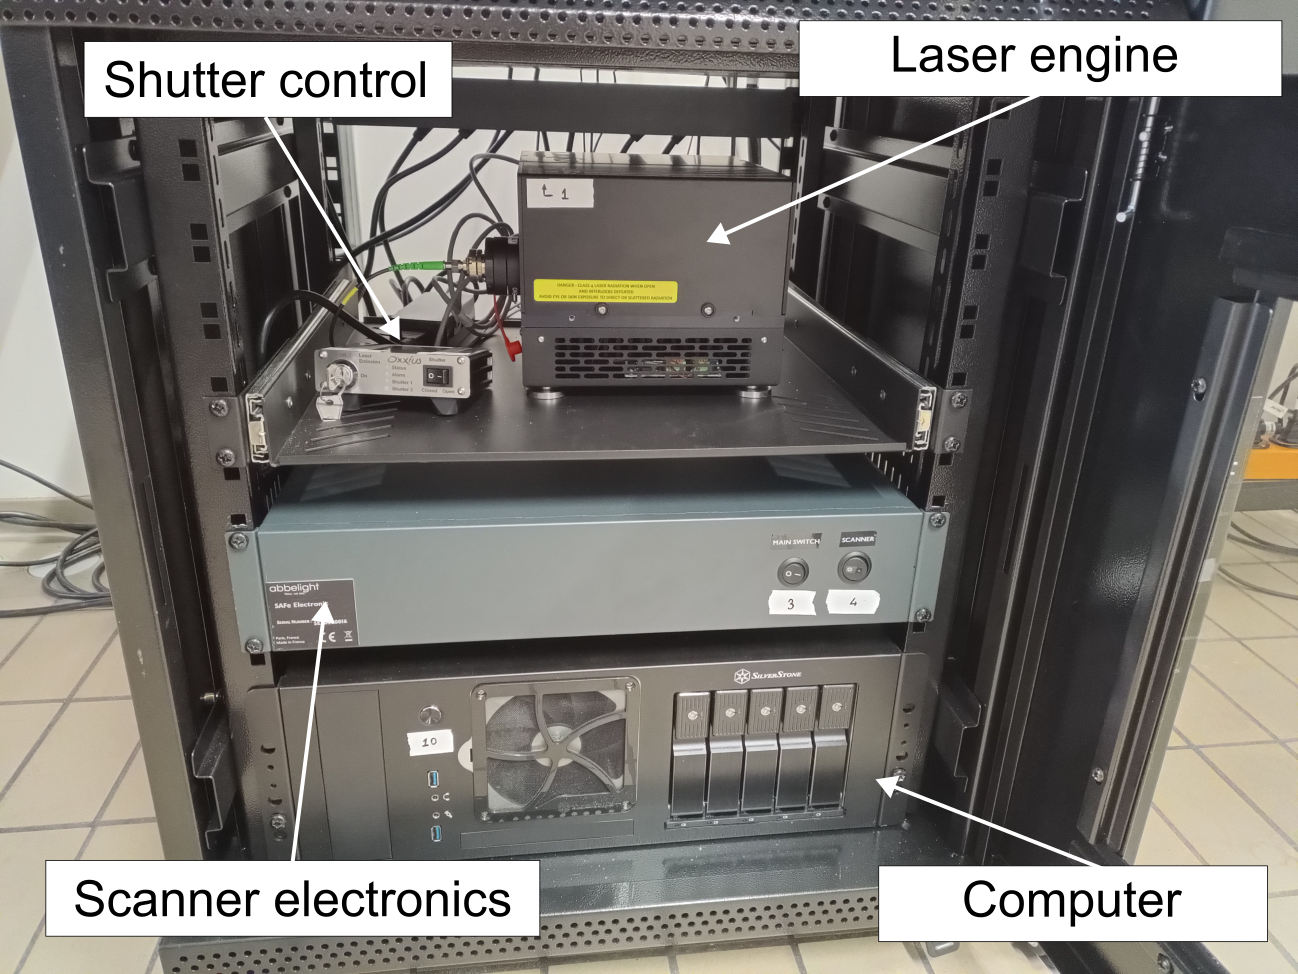
\includegraphics[width=0.75\textwidth]{electronics.png}
    \caption{Electronics and laser source for the microscope.}
    \label{fig:electronics}
\end{figure}

\section{Instrument Startup}\label{sec:startup}

To turn on the microscope, switch on the following components in this order. There should be pieces of tape with numbers on them and attached to the actual devices to aid you.

\begin{enumerate}
    \item Oxxius L4Cc laser engine
    \item Oxxius safety key
    \item Abbelight electronics: main switch
    \item Abbelight electronics: scanner
    \item Hamamatsu camera \newline Wait for the status light to turn green before proceeding.
    \item Olympus CBH microscope controller
    \item Maerhaeuser Tango Desktop stage controller
    \item Olympus control panel \newline Wait for the "Start Operation" button to appear, then press it to continue. This can take about one minute.
    \item Oxxius shutter
    \item The control computer
\end{enumerate}

\section{Instrument Shutdown}

Turn off the components in the opposite order as in \autoref{sec:startup}.

\end{document}
